\documentclass[tikz,border=50mm]{standalone}
% !TeX program = luatex

%===This is the preambule I call in every file===

\usepackage{tikz}
\usepackage{xcolor}
\usepackage{pgfplots}
\usepackage{circuitikz}
\usepackage{tikz-3dplot}
\pgfplotsset{compat=newest}
\usetikzlibrary{arrows.meta, shapes.geometric, positioning, perspective, patterns.meta, decorations.pathreplacing, decorations.pathmorphing, decorations.markings, patterns, arrows.meta, shapes, shapes.geometric, decorations.text, angles, quotes,calc, 3d, math, circuits.ee.IEC,hobby, knots, intersections, through}


%=== The Euler Med Logo ===
%=== i.e. My signature ===

\usepackage{amsmath, amsfonts}
\makeatletter
\newcommand*\eulermed{{
\scalebox{3.3}{$\mathbb{E}$}\kern-1pt \scalebox{1.5}{u$\ell\varepsilon\rho$}\kern-55pt
\raisebox{19pt}{\scalebox{1.5}{$\mathcal{M}\varepsilon\delta$}}}
\@}
\makeatother

\begin{document}
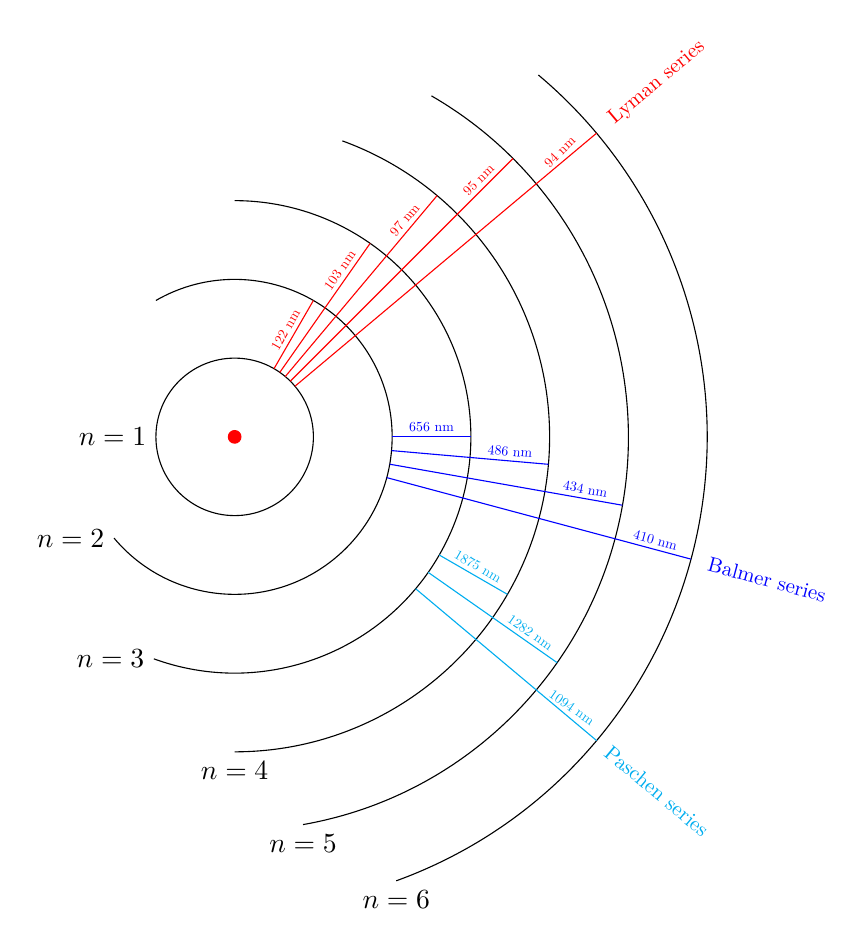
\begin{tikzpicture}[>=stealth]
%energy states
\filldraw[red] (0,0)circle(0.08);
\draw[smooth] (0,0)circle(1);
\node[left] at (180:1) {$n=1$};
\draw[smooth] (220:2)node[left] {$n=2$}arc(220:480:2);
\draw[smooth] (250:3)node[left] {$n=3$}arc(250:450:3);
\draw[smooth] (270:4)node[below] {$n=4$}arc(270:430:4);
\draw[smooth] (280:5)node[below] {$n=5$}arc(280:420:5);
\draw[smooth] (290:6)node[below] {$n=6$} arc(290:410:6);
%Lyman series 
\draw[red] (60:1)--(60:2) node[midway, above, rotate=60, scale=0.5] {$122$ nm};
\draw[red] (55:1)--(55:2) (55:2)--(55:3) node[midway, above, rotate=55,scale=0.5] {$103$ nm};
\draw[red] (50:1)--(50:3) (50:3)--(50:4) node[midway, above, rotate=50,scale=0.5] {$97$ nm};
\draw[red] (45:1)--(45:4) (45:4)--(45:5) node[midway, above, rotate=45,scale=0.5] {$95$ nm};
\draw[red] (40:1)--(40:5) (40:5)--(40:6) node[midway, above, rotate=45,scale=0.5] {$94$ nm};
\node[rotate=40, red, scale=0.75] at (40:7) {Lyman series};
%Balmer series
\draw[blue] (0:2)--(0:3) node[above, midway, scale=0.5] {656 nm};
\draw[blue] (-5:2)--(-5:3) (-5:3)--(-5:4)  node[above, midway, scale=0.5, rotate=-5] {486 nm};
\draw[blue] (-10:2)--(-10:4) (-10:4)--(-10:5)  node[above, midway, scale=0.5, rotate=-10] {434 nm};
\draw[blue] (-15:2)--(-15:5) (-15:5)--(-15:6)  node[above, midway, scale=0.5, rotate=-15] {410 nm};
\node[rotate=-15, blue, scale=0.75] at (-15:7) {Balmer series};
%Paschen series
\draw[cyan] (-30:3)--(-30:4)  node[above, midway, scale=0.5, rotate=-30] {1875 nm};
\draw[cyan] (-35:3)--(-35:4) (-35:4)--(-35:5)  node[above, midway, scale=0.5, rotate=-35] {1282 nm};
\draw[cyan] (-40:3)--(-40:5) (-40:5)--(-40:6)  node[above, midway, scale=0.5, rotate=-35] {1094 nm};
\node[rotate=-40, cyan, scale=0.75] at (-40:7) {Paschen series};
\end{tikzpicture}
\end{document}
